

\documentclass{uofa-eng-assignment}
\usepackage{caption}
\usepackage{hyperref}
\usepackage{tcolorbox}
\usepackage{boxedminipage}
\hypersetup{
    colorlinks = false,
    linkbordercolor = {white},
}
\captionsetup[table]{name=Tabla, labelsep=period}
\captionsetup[figure]{name=Figura, labelsep=period}

\newcommand{\hpl}{\hyperlink}
\newcommand{\hpt}{\hypertarget}
\newcommand*{\name}{Joan Sebastian Ramirez Sanchez}
\newcommand*{\id}{2223948}
\newcommand*{\course}{Introducción a la teoría de control}
\newcommand*{\assignment}[1]{Tarea #1}
\newcommand*{\dated}{\today}
\newcommand{\tf}{\textbf}

\begin{document}

\maketitle
\section*{Vehículo Aéreo No Tripulado Cuadricóptero}

\textbf{Contexto y aplicación.} 
Los cuadricópteros son plataformas de 6 grados de libertad (6-DOF) con fuerte acoplamiento no lineal. 
Su control preciso es esencial en logística autónoma, inspección de infraestructura y movilidad aérea urbana. Las no linealidades surgen de las transformaciones de orientación mediante ángulos de Euler

\subsection*{Variables del sistema}

\begin{center}
\begin{tabular}{lll}
\hline
\textbf{Símbolo} & \textbf{Unidades} & \textbf{Descripción} \\
\hline
$\phi, \theta, \psi$ & rad & Ángulos de Euler (roll, pitch, yaw) \\
$\Omega_i$ & rad/s & Velocidad angular del rotor $i$ \\
$k_T$ & N$\cdot$s$^2$ & Constante de empuje \\
$k_D$ & N$\cdot$m$\cdot$s$^2$ & Constante de par aerodinámico \\
$I_x, I_y, I_z$ & kg$\cdot$m$^2$ & Momentos de inercia principales \\
$L$ & m & Distancia del centro al rotor \\
\hline
\end{tabular}
\end{center}

\subsection*{Ecuaciones no lineales del sistema}

\begin{tcolorbox}[colback=brown!10!white, colframe=brown!60!black, title=No linealidades principales]
\begin{align*}
    \ddot{z} &= \frac{T}{m} \cos\phi \cos\theta - g 
\quad \text{(producto de trigonom.)} \\
I_x \ddot{\phi} 
&= \dot{\theta}\dot{\psi}(I_y - I_z) + \tau_\phi
\end{align*}
\end{tcolorbox}



%%%%%%%%%%%%%%%%%%%%%%%%%%%%%%%%%%%%%%%%%%%%%%%%%%%%%%%%%%%%%%%%%%
%%%%%%%%%%%%%%%%%%%%%%%%%%%%%%%%%%%%%%%%%%%%%%%%%%%%%%%%%%%%%%%%%%
%%%%%%%%%%%%%%%%%%%%%%%%%%%%%%%%%%%%%%%%%%%%%%%%%%%%%%%%%%%%%%%%%%
%%%%%%%%%%%%%%%%%%%%%%%%%%%%%%%%%%%%%%%%%%%%%%%%%%%%%%%%%%%%%%%%%%
%%%%%%%%%%%%%%%%%%%%%%%%%%%%%%%%%%%%%%%%%%%%%%%%%%%%%%%%%%%%%%%%%%

\section{Deducción matemática del sistema}

Un cuadricóptero es un vehículo aéreo no tripulado de seis grados de libertad (6-DOF): tres de posición $(x,y,z)$ y tres de orientación $(\phi,\theta,\psi)$. Su movimiento se describe mediante las leyes de Newton para la traslación del centro de masas y las ecuaciones de Euler para la rotación del cuerpo rígido.

\subsection{Fuerzas y pares generados por los rotores}

Cada rotor $i$ ($i=1,2,3,4$) gira con velocidad angular $\Omega_i$ y produce:
\begin{itemize}
    \item Una fuerza de empuje perpendicular al plano del rotor: $F_i = k_T\,\Omega_i^2$.
    \item Un par de reacción aerodinámico opuesto al giro: $M_i = k_D\,\Omega_i^2$.
\end{itemize}

El empuje total $T$ y los pares netos que actúan sobre el vehículo se obtienen combinando las contribuciones de los cuatro rotores. En una configuración simétrica (cruz o X) se tiene típicamente
\begin{align}
    T      &= k_T(\Omega_1^2+\Omega_2^2+\Omega_3^2+\Omega_4^2), \label{eq:empuje}\\
    \tau_\phi &= L\,k_T(\Omega_4^2-\Omega_2^2), \label{eq:roll}\\
    \tau_\theta &= L\,k_T(\Omega_1^2-\Omega_3^2), \label{eq:pitch}\\
    \tau_\psi   &= k_D(\Omega_1^2-\Omega_2^2+\Omega_3^2-\Omega_4^2), \label{eq:yaw}
\end{align}
donde $L$ es la distancia del centro de masas a cada rotor. En este trabajo nos centramos exclusivamente en el control de la altitud $z$ y del ángulo de alabeo (\textit{roll}) $\phi$, por lo que las entradas de control que aparecerán en el modelo son el empuje total $T$ y el par de roll $\tau_\phi$.

\subsection{Dinámica de traslación (altitud)}

La segunda ley de Newton aplicada al centro de masas en el sistema de referencia inercial se escribe
\[
m\,\ddot{\mathbf{r}} = \mathbf{F}_{\text{empuje}} + \mathbf{F}_{\text{gravedad}}.
\]

El empuje total $T$ está dirigido a lo largo del eje $z$ del cuerpo del dron. Para expresarlo en coordenadas inerciales se utiliza la matriz de rotación $R$ definida por los ángulos de Euler (convención $ZYX$):
\[
R = R_z(\psi)\,R_y(\theta)\,R_x(\phi).
\]

La componente vertical (inercial) de la fuerza de empuje es entonces $T\cos\phi\cos\theta$. La fuerza de gravedad actúa hacia abajo, $\mathbf{F}_g = -mg\,\hat{\mathbf{k}}$. Por tanto, la ecuación de movimiento para la altura $z$ resulta
\begin{equation}
\boxed{\ddot{z} = \frac{T}{m}\cos\phi\cos\theta - g}. \label{eq:z}
\end{equation}

Las ecuaciones análogas para las coordenadas horizontales $x$ e $y$ no se incluyen en este subsistema simplificado.

\subsection{Dinámica de rotación (roll)}

La evolución de la orientación del cuerpo rígido está gobernada por las ecuaciones de Euler
\[
\mathbf{I}\,\dot{\boldsymbol{\omega}} = -\boldsymbol{\omega}\times(\mathbf{I}\boldsymbol{\omega}) + \boldsymbol{\tau},
\]
donde $\boldsymbol{\omega}=[p,q,r]^T$ es el vector de velocidades angulares en ejes cuerpo (roll, pitch y yaw, respectivamente), $\mathbf{I}=\operatorname{diag}(I_x,I_y,I_z)$ es la matriz de inercia y $\boldsymbol{\tau}=[\tau_\phi,\tau_\theta,\tau_\psi]^T$ son los pares aplicados.

Para ángulos pequeños, las velocidades angulares se aproximan por las derivadas de los ángulos de Euler:
\[
p \approx \dot{\phi},\qquad q \approx \dot{\theta},\qquad r \approx \dot{\psi}.
\]

Tomando la primera componente de la ecuación de Euler (eje $x$ del cuerpo) se obtiene
\[
I_x\,\dot{p} = q\,r\,(I_y - I_z) + \tau_\phi.
\]

Sustituyendo las aproximaciones anteriores llegamos a la dinámica no lineal del ángulo de roll:
\begin{equation}
\boxed{I_x\,\ddot{\phi} = \dot{\theta}\dot{\psi}(I_y - I_z) + \tau_\phi}. \label{eq:phi}
\end{equation}

\subsection{Modelo no lineal de partida}

Las ecuaciones \eqref{eq:z} y \eqref{eq:phi} constituyen el modelo reducido con el que trabajaremos:
\[
\begin{aligned}
\ddot{z}      &= \frac{T}{m}\cos\phi\cos\theta - g,\\
I_x\ddot{\phi}&= \dot{\theta}\dot{\psi}(I_y - I_z) + \tau_\phi.
\end{aligned}
\]

Las no linealidades provienen de los productos trigonométricos ($\cos\phi\cos\theta$) y del acoplamiento giroscópico ($\dot{\theta}\dot{\psi}(I_y-I_z)$). En la Sección~3 se linealizará este sistema alrededor de un punto de equilibrio adecuado.
%%%%%%%%%%%%%%%%%%%%%%%%%%%%%%%%%%%%%%%%%%%%%%%%%%%%%%%%%%%%%%%%%%
%%%%%%%%%%%%%%%%%%%%%%%%%%%%%%%%%%%%%%%%%%%%%%%%%%%%%%%%%%%%%%%%%%
%%%%%%%%%%%%%%%%%%%%%%%%%%%%%%%%%%%%%%%%%%%%%%%%%%%%%%%%%%%%%%%%%%
%%%%%%%%%%%%%%%%%%%%%%%%%%%%%%%%%%%%%%%%%%%%%%%%%%%%%%%%%%%%%%%%%%


\section{Punto de equilibrio}
Para hallar el punto de equilibrio del sistema, buscamos las condiciones de vuelo estacionario (hovering). 
Esto implica que el vehículo se encuentra en una posición fija, sin velocidades ni aceleraciones lineales o angulares
por lo tanto debemos tener
\begin{itemize}
    \item aceleraciones lineales nulas: $\ddot{z}=\ddot{\phi}=\ddot{\theta}=\ddot{\psi}=0$
    \item velocidades lineales nulas: $\dot{z}=\dot{\phi}=\dot{\theta}=\dot{\psi}=0$
\end{itemize}
Además que necesitamos que la orientación del "dron" sea tal que no este desbalanceado entonces 
necesitamos que $\phi=\theta=0$ dado que son los ángulos de roll y pitch respectivamente, 
entonces el único ángulo que puede ser diferente de cero es el yaw $\psi$ 
pero dado que no afecta a la dinámica del sistema entonces podemos asumir que $\psi=0$ 
sin perdida de generalidad, por lo tanto el punto de equilibrio del sistema 
es (\textbf{explicar que es roll y pitch en la sección 1})
por lo tanto haciendo el análisis de las ecuaciones diferenciales del sistema entonces tenemos que el punto de equilibrio es
\begin{align*}
    0= \frac{T}{m} \cos 0 \cos 0 - g \implies T=mg
\end{align*}
esto para la ecuación diferencial de la aceleración lineal en el eje z, 
y para las ecuaciones diferenciales de las aceleraciones angulares entonces tenemos que
\begin{align*}
    0 = \dot{\theta}\dot{\psi}(I_y - I_z) + \tau_\phi \implies \tau_\phi=0 \\
\end{align*}
Viéndolo de manera vectorial el punto de equilibrio será 
\begin{align*}
    z_e = z_0 , \quad
    \dot{z}_e = 0, \\ 
    \phi_e = 0, \quad
    \theta_e=0, \\
    \psi_e = 0, \quad
    \dot{\phi_e}=0,\\
    \dot{\theta_e}=0, \quad
    \dot{\psi_e}=0,\\
\end{align*}
%%%%%%%%%%%%%%%%%%%%%%%%%%%%%%%%%%%%%%%%%%%%%%%%%%%%%%%%%%%%%%%%%%
%%%%%%%%%%%%%%%%%%%%%%%%%%%%%%%%%%%%%%%%%%%%%%%%%%%%%%%%%%%%%%%%%%
%%%%%%%%%%%%%%%%%%%%%%%%%%%%%%%%%%%%%%%%%%%%%%%%%%%%%%%%%%%%%%%%%%
%%%%%%%%%%%%%%%%%%%%%%%%%%%%%%%%%%%%%%%%%%%%%%%%%%%%%%%%%%%%%%%%##





\section{Linealización del sistema}
Vamos a linealizar el sistema alrededor del punto de equilibrio encontrado en la sección anterior,
para esto definiremos las siguientes variables
\begin{align*}
    \delta z = z -z_e,& \quad \delta \dot{z}= \dot{z}-0, \delta \phi = \phi - 0, \quad \delta \dot{\phi} = \dot{\phi}\\
&\delta T = T-mg, \quad \delta \tau_\phi = \tau_\phi - 0,
\end{align*}
Se considerará tambien que $\delta \theta = \theta, \delta \psi = \psi, \delta \dot{\theta} = \dot{\theta}, \delta \dot{\psi} = \dot{\psi}$, Como este modelo no tiene estas ecuaciones supondremos que están equilibrio (cero), o cualquier caso las su atribuciones serán nulas.
\begin{align*}
    \delta \dot{z} \approx \frac{\partial}{\partial T}\Big|_{z_e} \Delta T + \frac{\partial}{\partial \phi} \Big|_{z_e} \Delta \phi + \frac{\partial }{\partial \theta} \Big|_{z_e} \Delta \theta 
\end{align*}
Dónde 
\begin{align*}
    \frac{\partial}{\partial T}=\frac{1}{m} cos \phi cos \theta \Big|_{z_e}=\frac{1}{m}\\
    \frac{\partial}{\partial \phi}= -\frac{T}{m} \sin \phi \cos \theta \Big|_{z_e} = 0 \\
    \frac{\partial}{\partial \theta} = -\frac{T}{m} \cos \phi \sin \theta \Big|_{z_e} = 0 
\end{align*}
Por lo tanto
\[
\delta \ddot{z} \approx \frac{1}{m}\delta T
\]
eso para la primera ecuación diferencial, para la segunda ecuación tenemos lo siguiente 
\begin{align*}
    \delta \ddot{\phi} \approx \frac{\partial}{\partial \dot{\theta}} \Big|_{z_e} \Delta \dot{\theta} + \frac{\partial}{\partial \dot{\psi}} \Big|_{z_e} \Delta \dot{\psi} + \frac{1}{I_x} \delta \tau_\phi 
\end{align*}
y 
\begin{align*}
    \frac{\partial}{\partial \dot{\theta}} = \frac{\dot{\psi} I_y-I_z}{I_x}\Big|_{z_e} = 0, \quad \frac{\partial}{\partial \dot{\psi}}= \frac{\dot{\theta}(I_y-I_z)}{I_x}\Big|_{z_e} = 0  
\end{align*}
Resulta \[
\delta \ddot{\phi} = \frac{1}{I_x} \delta \tau_\phi\]
ahora tomando como vector de estados $x=[\delta z, \delta \dot{z}, \delta \phi, \delta \dot{\phi}]$ y el vector de control de entrada $u=[\delta T, \delta \tau_\phi]$ entonces tenemos que

\begin{align*}
    \dot{x} = \begin{bmatrix}
        \delta \dot{z} \\
        \delta \ddot{z} \\
        \delta \dot{\phi} \\
        \delta \ddot{\phi}
    \end{bmatrix}  = \begin{bmatrix}
        0 & 1 & 0 & 0 \\
        0 & 0 & 0 & 0 \\
        0 & 0 & 0 & 1 \\
        0 & 0 & 0 & 0
    \end{bmatrix}
    \begin{bmatrix}
        \delta z \\
        \delta \dot{z} \\
        \delta \phi \\
        \delta \dot{\phi}
    \end{bmatrix} + \begin{bmatrix}
        0 & 0 \\
        \frac{1}{m} & 0 \\
        0 & 0 \\
        0 & \frac{1}{I_x}
    \end{bmatrix}
    \begin{bmatrix}
        \delta T \\
        \delta \tau_\phi
    \end{bmatrix}
\end{align*}
\section{Solución del sistema linealizado}
Dado que el modelo es $\dot{x} = Ax+Bu$, entonces tenemos que la solución será de la forma
\begin{align*}
    x = e^{At} x(0) + \int_0^t e^{A(t-s)} B  u(s) ds  
\end{align*}
con \begin{align*}
    x = \begin{bmatrix}
        \delta \dot{z} \\
        \delta \ddot{z} \\
        \delta \dot{\phi} \\
        \delta \ddot{\phi}
    \end{bmatrix}, \quad A = \begin{bmatrix}
        0 & 1 & 0 & 0 \\
        0 & 0 & 0 & 0 \\
        0 & 0 & 0 & 1 \\
        0 & 0 & 0 & 0
    \end{bmatrix}
, \quad B = \begin{bmatrix}
        0 & 0 \\
        \frac{1}{m} & 0 \\
        0 & 0 \\
        0 & \frac{1}{I_x}
    \end{bmatrix}
\end{align*}
Viendo que la matriz $A$ es un matriz nilpotente entonces la forma exponencial de la matriz es más fácil
observe que: 
\begin{align*}
    A ^2 = \begin{bmatrix}
        0& 0 & 0 & 0 \\
        0& 0 & 0 & 0 \\
        0& 0 & 0 & 0 \\
        0& 0 & 0 & 0 
    \end{bmatrix}
\end{align*}
Por lo tanto la matriz exponencial de $A$ será
\begin{align*}
    e^{At} = I+ At = \begin{bmatrix}
        1 & t & 0 & 0 \\
        0 & 1 & 0 & 0 \\
        0 & 0 & 1 & t \\
        0 & 0 & 0 & 1 \\
    \end{bmatrix}
\end{align*}
en forma matricial tenemos la solución del sistema linealizado es
\begin{align*}
    \begin{bmatrix}
    \delta z(t) \\
    \delta \dot{z}(t) \\
    \delta \phi(t) \\
    \delta \dot{\phi}(t)
    \end{bmatrix}= \begin{bmatrix}
                1 & t & 0 & 0 \\
        0 & 1 & 0 & 0 \\
        0 & 0 & 1 & t \\
        0 & 0 & 0 & 1 \\
    \end{bmatrix} \begin{bmatrix}
        \delta z(0) \\
        \delta \dot{z}(0) \\
        \delta \phi(0) \\
        \delta \dot{\phi}(0)
    \end{bmatrix} + \int_0^t \begin{bmatrix}
        1 & t & 0 & 0 \\
        0 & 1 & 0 & 0 \\
        0 & 0 & 1 & t \\
        0 & 0 & 0 & 1 \\
    \end{bmatrix} \begin{bmatrix}
        0 & 0 \\
        \frac{1}{m} & 0 \\
        0 & 0 \\
        0 & \frac{1}{I_x}
    \end{bmatrix} \begin{bmatrix}
        \delta T(s) \\
        \delta \tau_\phi(s)
    \end{bmatrix} ds
\end{align*}
Y de una manera mas desglosada la solución del sistema será
\begin{align*}
    \delta z(t) = \delta z(0)+ t \delta \dot{z}(0)+ \frac{1}{m}\int_0^t (t-s)\delta T(s) ds \\
    \delta \dot{z}(t) = \delta \dot{z}(0) + \frac{1}{m}\int_0^t \delta T(s) ds 
\end{align*}
\[
\delta \phi(t)
=
\delta \phi(0)
+
t\,\delta \dot{\phi}(0)
+
\frac{1}{I_x}
\int_{0}^{t}
(t-\tau)\,\delta \tau_{\phi}(\tau)\, d\tau,
\]

\[
\delta \dot{\phi}(t)
=
\delta \dot{\phi}(0)
+
\frac{1}{I_x}
\int_{0}^{t}
\delta \tau_{\phi}(\tau)\, d\tau.
\]
\begin{figure}[h]
    \centering
    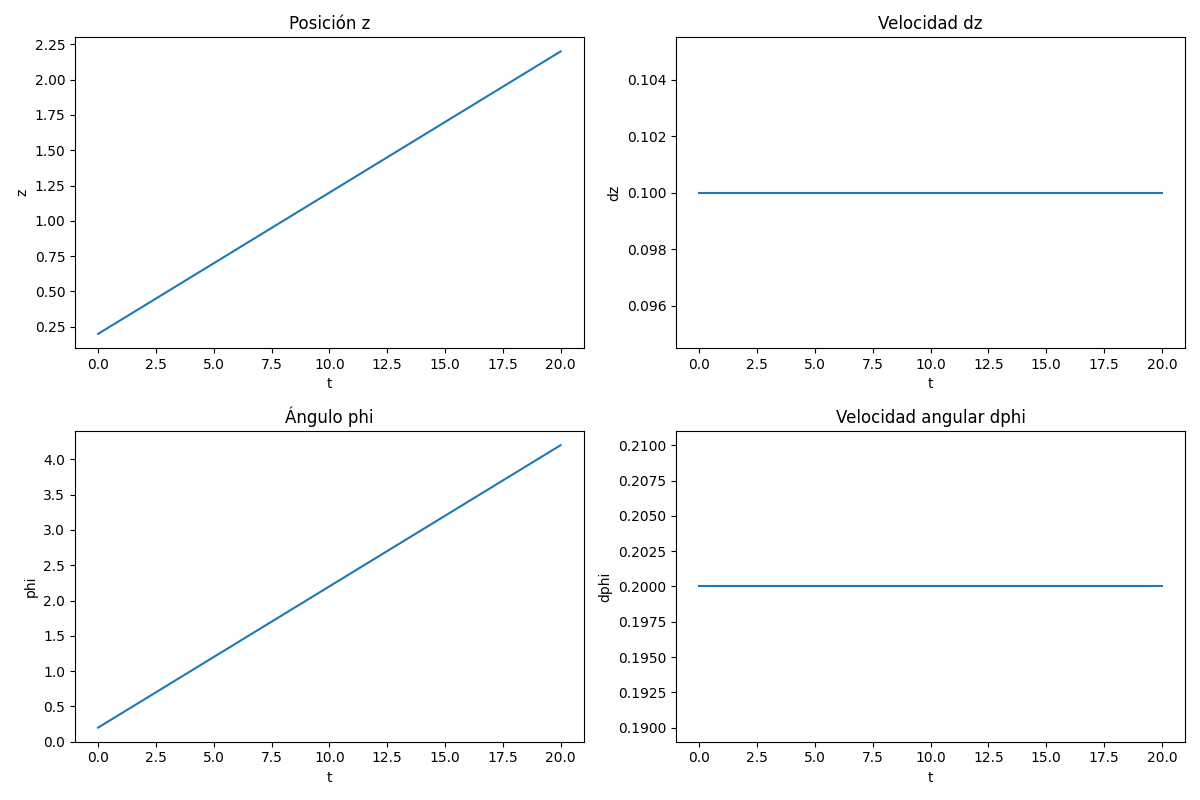
\includegraphics[width=0.8\textwidth]{graficasinforzante.png}
    \caption{Evolución de los estados del sistema linealizado con una entrada de control nula y un estado inicial dado}
\end{figure}
\section{Controlabilidad del sistema}
Ver si el sistema es controlable vamos a hacer uso del teorema de Kalman y dado que nuestra matriz $A$ es
nilpotente entonces tenemos los siguiente
 \[
 \mathcal{C} = [B,AB]
 \]
 donde 
 \[
 A= \begin{bmatrix}
        0 & 1 & 0 & 0 \\
        0 & 0 & 0 & 0 \\
        0 & 0 & 0 & 1 \\
        0 & 0 & 0 & 0
    \end{bmatrix}, \quad AB = \begin{bmatrix}
        0 & 0 \\
        \frac{1}{m} & 0 \\
        0 & 0 \\
        0 & \frac{1}{I_x}
    \end{bmatrix}
 \]
 Asi $\mathcal{C}$ es 
  \[
\begin{bmatrix}
0 & 0 & \frac{1}{m} & 0 & 0 & 0 & 0 & 0 \\
\frac{1}{m} & 0 & 0 & 0 & 0 & 0 & 0 & 0 \\
0 & 0 & 0 & \frac{1}{I_x} & 0 & 0 & 0 & 0 \\
0 & \frac{1}{I_x} & 0 & 0 & 0 & 0 & 0 & 0
\end{bmatrix}
\]

 Por lo tanto $Rank(\mathcal{C})= 4$  dado que todas sus filas son linealmente independientes entonces el sistema es controlable
\section{Conjunto de datos admisibles}
Dado que no hay restricciones en las entradas, cualquier vector de estado inicial puede ser llevado al origen (o a cualquier estado 
deseado) en un tiempo finito, por lo tanto el conjunto de datos iniciales admisibles es $\mathbb{R}^4$.

\section{Control en un tiempo dado}
Vamos a separar este proceso en según las ecuaciones que estamos trabajando dado que como podemos ver la solución
depende de la altura y su aceleración y del angulo y su aceleración osea que podemos coger por pares comenzando 
por la altura la cual la podemos ver de este modo
\begin{align*}
    \frac{d}{dt}
    \begin{bmatrix}
        x_1 \\
        x_2 \\
    \end{bmatrix}
    = \begin{bmatrix}
        0 & 1 \\
        0 & 0
    \end{bmatrix}\begin{bmatrix}
        x_1 \\
        x_2 \\
    \end{bmatrix} + 
    \begin{bmatrix}
    0 \\
     \frac{1}{m} 
    \end{bmatrix}
    u
\end{align*}
dónde 
\[
x_1 = \delta z, \quad x_2 = \delta \dot{z}, \quad u = \delta T, m \text{ es la masa del cuadricóptero}
\]
sus ecuaciones diferenciales son 
\[
\dot{x}_1 = x_2 , \quad \dot{x}_2= \frac{u}{m}
\]
dando un estado inicial $(x_1(0),x_2(0))= (\delta z_0, \delta \dot{z}_0)$ y un tiempo final $T >0$ queremos hallar una función $u(t)$
tal que el estado llegue al origen en $t= T$
\[
x_1(T) = 0, x_2(T)=0
\]
y para encontrar el control haremos uso de la siguiente formula, que aparece en las notas de clase.
\[
\bar{u}(s) := \left( e^{(T-s)A} B \right)^T G^{-1} \left( y_T - e^{(T-s)A} y_0 \right),
\tag{2.12}
\]
con 
\[
G = \int_{0}^{T} \left( e^{tA} B \right) \left( e^{tA} B \right)^T dt
\]
Calculando la exponencial, como es exponencial es fácil su calculo
\[
e^At = I+At = \begin{bmatrix}
    1 & t \\
    0 & 1
\end{bmatrix}
\]
Asi tenemos que $e^{(T-s)A}$ es 
\[
e^{(T-s)A} = \begin{bmatrix}
    1 & T-s \\
    0 & 1
\end{bmatrix}
\]
Por lo tanto transponiendo, el termino $(e^{(T-s)A}B)^T$, nos queda algo asi,

\[
 (e^{(T-s)A}B)^T= 
\begin{bmatrix}
  \frac{T-s}{m}  &
  \frac{1}{m}
\end{bmatrix}
\]
Voy a poner el calculo de $G$ dado que si no extenderiamos demasiado los cálculos 
\[
G^{-1} = m^2
\begin{pmatrix}
\frac{12}{T^3} & -\frac{6}{T^2} \\
-\frac{6}{T^2} & \frac{4}{T}
\end{pmatrix}
\]
para calcular $d = \left( x_T - e^{(T-s)A} y_0 \right),$
\[
e^{A^T} x_0 =
\begin{bmatrix}
1 & T \\
0 & 1
\end{bmatrix}
\begin{bmatrix}
\delta z_0 \\
\dot{\delta z}_0
\end{bmatrix}
=
\begin{bmatrix}
\delta z_0 + T \dot{\delta z}_0 \\
\dot{\delta z}_0
\end{bmatrix},
\]

\[
d =
\begin{bmatrix}
0 \\
0
\end{bmatrix}
-
\begin{bmatrix}
\delta z_0 + T \dot{\delta z}_0 \\
\dot{\delta z}_0
\end{bmatrix}
=
\begin{bmatrix}
- \delta z_0 - T \dot{\delta z}_0 \\
- \dot{\delta z}_0
\end{bmatrix}.
\]
Por lo tanto tenemos que 
\begin{align*}
    \tilde{u}(s)= \begin{bmatrix}
  \frac{T-s}{m}  &
  \frac{1}{m}
\end{bmatrix} \cdot m^2\begin{pmatrix}
\frac{12}{T^3} & -\frac{6}{T^2} \\
-\frac{6}{T^2} & \frac{4}{T}
\end{pmatrix}\begin{bmatrix}
- \delta z_0 - T \dot{\delta z}_0 \\
- \dot{\delta z}_0
\end{bmatrix}.
\end{align*}
Haciendo algunos cálculos

\[
\tilde{u}(s) = 
\left[ \frac{T - s}{m} \;\; \frac{1}{m} \right] 
\cdot m^2
\begin{bmatrix}
-\frac{12}{T^3} \delta z_0 & -\frac{6}{T^2} \dot{\delta z}_0 \\
\frac{6}{T^2} \delta z_0 & \frac{4}{T} \dot{\delta z}_0
\end{bmatrix}
\]


\begin{align*}
\tilde{u}(s) &= m(T-s) 
\begin{pmatrix}
-\frac{12}{T^3} \delta z_0 & -\frac{6}{T^2} \dot{\delta z}_0
\end{pmatrix}
+ m
\begin{pmatrix}
\frac{6}{T^2} \delta z_0 & \frac{2}{T} \dot{\delta z}_0
\end{pmatrix} \\
&= m \begin{pmatrix}
-\frac{12(T-s)}{T^3} \delta z_0 - \frac{6(T-s)}{T^2} \dot{\delta z}_0
+ \frac{6}{T^2} \delta z_0 + \frac{2}{T} \dot{\delta z}_0
\end{pmatrix} \\
&= m \begin{pmatrix}
\left(-\frac{12(T-s)}{T^3} + \frac{6}{T^2}\right) \delta z_0 +
\left(-\frac{6(T-s)}{T^2} + \frac{2}{T}\right) \dot{\delta z}_0
\end{pmatrix} \\
\end{align*}
Simplificando los coeficientes:
\begin{align*}
    \delta z_0: &\quad -\frac{12T}{T^3} + \frac{12s}{T^3} + \frac{6}{T^2} 
= \frac{12s - 6T}{T^3} \\ 
\dot{\delta z}_0: &\quad -\frac{6T}{T^2} + \frac{6s}{T^2} + \frac{2}{T} 
= \frac{6s - 4T}{T^2}
\end{align*}
por lo tanto el control es 
\[
\tilde{u}(s) = \delta T(s) = m
\begin{bmatrix}
\dfrac{12s - 6T}{T^3} \, \delta z_0 + \dfrac{6s - 4T}{T^2} \, \dot{\delta z}_0
\end{bmatrix}
\]
De la misma manera, pero sin complicarnos hay que hacer los cálculos para el angulo (roll) ya que solo hay que cambiar $m$ por $I_x$
tenemos que  
\[
\delta_{\tau \phi}(s) = I_x
\begin{bmatrix}
\dfrac{12s - 6T}{T^3} \, \delta \phi_0 + \dfrac{6s - 4T}{T^2} \, \dot{\delta \phi}_0
\end{bmatrix}.
\]
usando los siguientes parámetros 
\begin{itemize}
    \item $m = 0.5~\text{kg}, \quad I_x = 0.02~\text{kg}\cdot\text{m}^2$
    \item $T = 2~\text{s}$
    \item Estado inicial: $\delta z_0 = 2~\text{m}, \;\; \dot{\delta z}_0 = 0.5~\text{m/s}, \;\; \delta \phi_0 = 0.2~\text{rad}, \;\; \dot{\delta \phi}_0 = -0.1~\text{rad/s}$
\end{itemize}
tenemos que
 \begin{figure}[h]
    \centering
    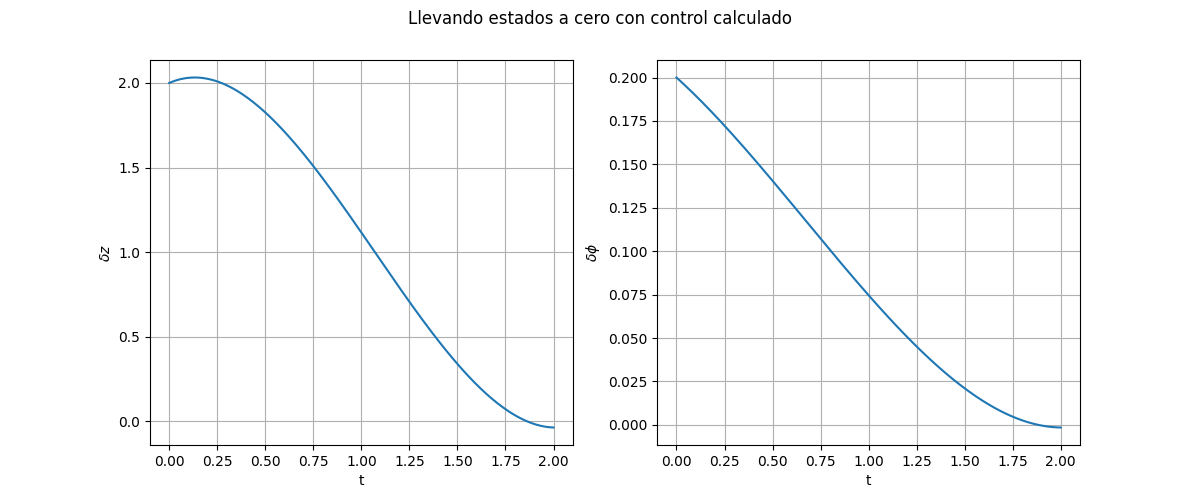
\includegraphics[width=0.8\textwidth]{graficacontorl.png}
    \caption{Control de entrada para llevar el sistema al origen en $T=2$ segundos}
 \end{figure}

\end{document}
